%% -*- Lecture -*-

\documentclass[11pt,aspectratio=169]{beamer}

\usepackage{rcstalk}
\usetheme{rcstheme}

\usepackage{tikzpeople}

\topic{Introduction}

%\title{CS350: Operating Systems\\
%Introduction}

\begin{document}

\tikzstyle{osbox}=[draw, fill=blue!20, text width=20em, text centered, minimum 
height=2em]
\tikzstyle{hwbox}=[draw, fill=green!20, text width=20em, text centered, minimum 
    height=2em]
\tikzstyle{appbox}=[draw, fill=white, text width=5em, text centered, minimum 
    height=2em]
\def\blockdist{0.5}

\maketitle

\section{Administrative}

\begin{slide}{Administrivia}
\itms{
  \item Class web page: \url{https://student.cs.uwaterloo.ca/~cs350/}
  \ittms{
    \item All assignments, lecture notes and handouts
  }
  \gap
  \item Textbooks
  \ittms{
    \item \emph{Operating System Concepts}
    %, by Silberschatz, Galvin, and Gagne
    \item \emph{Operating Systems: Three Easy Pieces}
    %, by Remzi and Andrea
  }
}
\end{slide}

\begin{slide}{Administrivia Continued}
\itms{
  \item Q\&A through Piazza (see class website)
  \item Assignment help primarily through Office hours
  \gap
  \item Midterm is scheduled for October 30, 2024
  \item Final will be announced later
  \gap
  \item Four projects due throughout term
  \item One extra credit reading assignment
}
\end{slide}

\begin{slide}{Improvements and Changes to the Material}
\itms{
\item Slides and course content changes
\ittms{
    \item Removing some examples and details
    \item Expanding the slides where we think students struggled the most
}
\gap
\item Assignment documents and code have been updated.
\ittms{
    \item Numerous improvements to the code
    \item Improve the compatability across different build environments
    \item Improved write-ups (will be released next week)
}
\gap
\item Expanding the in-class assignments
\ittms{
    \item Designed to make the ideas from lecture more concrete
    \item Solutions will not be provided outside of lecture
}
}
\end{slide}

\begin{slide}{How to do well in CS350}
\itms{
\item Attend lecture
    \ittms{
    \item Course notes are updated every term
    \item You are responsible for this terms course material
    \item Watching videos from older terms {\bf is not} a substitute
    }
\item Complete the assignments:
    \ittms{
    \item {\em Read} the assignments in detail
    \item Complete the assignments
    \item Ask yourself if you understand what your doing? (Good piazza 
	discussion!)
    \item Usually we test material from the assignments!
    }
\item Complete the reading assignments:
    \ittms{
    \item Reading assignments are a great resource
    \item Both texts can expand and clarify topics
    }
}
\end{slide}

\section{Why study operating systems?}

\begin{slide}{Course Goals: Introduce you to Systems}
\itms{
  \item Operating Systems
  \item Distributed Systems
  \item Networking
  \item Internet of Things
  \item Computer Architecture
  \item Embedded Systems
  \item Database Systems
  \item Systems and Machine Learning
  \item ...
}
\end{slide}

\begin{slide}{Course Goals: A Computer Systems Way of Thinking}
\itms{
\item Make sense of complex software
\ittms{
    \item Think in terms of the whole system or major components
    \item Analyze the properties of the whole system
}
\gap
\item Practical tools for designing and improving software
\gap
\item Practical prinicples for designing and improving software
}
\end{slide}

\begin{slide}{Course Goals: Practical Understanding of OSes}
\itms{
  \item Introduce you to operating systems
  \ittms{
    \item Every computer, phone and smart watch runs an OS
    \item Makes you a more effective programmer
    \item How the OS affects your software
  }
  \gap
  \item General systems concepts
  \ittms{
    \item Concurrency, memory management, and I/O
    \item Security and protection
    \item Tools for software performance
  }
  \gap
  \item Practical skills
  \ittms{
    \item Learn to work with large code bases
    \item My lectures: industry and research experience
  }
}
\end{slide}

%\begin{slide}{What is an operating system?}
\begin{frame}
\frametitle{What is an operating system?}
\itms{
\item Layer between applications and hardware \\
%\centerline{\includegraphics[width=3in]{figs/whatis}}

\begin{figure}[ht!]
\centering
\begin{tikzpicture}
    \node (os) [osbox] {Operating System};
    \path (os.south)+(0,-\blockdist) node (hw) [hwbox] {Hardware: CPU, Memory 
    and Devices};
    \path (os.north)+(0,\blockdist) node (emacs) [appbox,fill=yellow!30] 
    {emacs};
    \path (os.north)+(-6em,\blockdist) node (emacs) [appbox,fill=black!30] 
    {gcc};
    \path (os.north)+(6em,\blockdist) node (emacs) [appbox,fill=red!30] {Doom};
\end{tikzpicture}
\end{figure}

\item Makes hardware useful to the programmer
 \item Usually: Provides abstractions for applications
  \ittms{
   \item Manages and hides details of hardware
   \item Accesses hardware through low/level interfaces unavailable to
     applications
  }
 \item Often: Provides protection
  \ittms{
   \item Prevents one process/user from clobbering another
  }
}
\end{frame}

\begin{slide}{Why study operating systems?}
\itms{
  \item Operating systems are a maturing field
  \ittms{
    \item Most people use a handful of mature OSes
    \item Hard to get people to switch operating systems
    \item Hard to have impact with a new OS
  }
  \item High-performance servers are an OS issue
  \ittms{
    \item Face many of the same issues as OSes
  }
  \item Resource consumption is an OS issue
  \ittms{
    \item Battery life, radio spectrum, etc.
  }
  \item Security is an OS issue
  \ittms{
    \item Security requires a solid foundation
  }
  \item New ``smart'' devices need new OSes
  \item Web browsers, databases, and game engines look like OSes
}
\end{slide}

\section{Course overview}

\begin{slide}{Course topics}
\itms{
  \item Threads \& Processes
  \item Concurrency \& Synchronization
  \item Scheduling
  \item Virtual Memory
  \item I/O
  \item Disks, File systems, Network file systems
  \item Protection \& Security
  \item Virtual machines
  \item Will often use Unix as the example
  \ittms{
    \item Most OSes heavily influenced by Unix (including the assignment)
    \item Windows is a notable exception
  }
}
\end{slide}

\begin{slide}{Primitive Operating Systems}
\itms{
  \item Just a library of standard services (no protection)
    %\item[] \includegraphics[width=2.5in]{figs/os0}

\begin{figure}[ht!]
\centering
\begin{tikzpicture}
    \node (hw) [hwbox] {Hardware: CPU, Memory and Devices};
    \path (hw.north)+(0,3em) node (emacs) [appbox,text width=10em, minimum 
    height=5.5em, fill=yellow!30] {IoT Sensor\\};
    \path (emacs)+(0.85,-0.6) node (libos) [osbox,text width=5em] {Library OS};
\end{tikzpicture}
\end{figure}

  \ittms{
    \item Standard interface above hardware-specific drivers, etc.
  }
  \item Simplifying assumptions
  \ittms{
    \item System runs one program at a time
    \item No bad users or programs (often bad assumption)
  }
  \item Problem:  Poor utilization
  \ittms{
    \item \ldots of hardware (e.g., CPU idle while waiting
    for disk)
    \item \ldots of human user (must wait for each program to finish)
  }
}
\end{slide}

\begin{frame}
\frametitle{Multitasking}
%\centerline{\includegraphics[width=3in]{figs/os1}}

\begin{figure}[ht!]
\centering
\begin{tikzpicture}
    \node (os) [osbox] {Operating System};
    \path (os.south)+(0,-\blockdist) node (hw) [hwbox] {Hardware: CPU, Memory 
    and Devices};
    \path (os.north)+(3em,\blockdist) node (emacs) [appbox,fill=yellow!30] 
    {emacs};
    \path (os.north)+(-3em,\blockdist) node (emacs) [appbox,fill=black!30] 
    {gcc};
\end{tikzpicture}
\end{figure}

\itms{
  \item Idea:  Run more than one process at once
  \ittms{
    \item When one process blocks (waiting for user
	  input, IO, etc.)\ run another process
  }
  \item Problem:  What can ill-behaved process do?
\pause
  \ittms{
    \item Go into infinite loop and never relinquish CPU
    \item Scribble over other processes' memory to make them fail
  }
  \item OS provides mechanisms to address these problems
  \ittms{
    \item \emph{Preemption} -- take CPU away from looping process
    \item \emph{Memory protection} -- protect process's memory from
  one another
  }
}
\end{frame}

\begin{slide}{Multi-user OSes}
%\centerline{\includegraphics[height=1.3in]{figs/os2}}

\vspace{-1em}
\begin{figure}[ht!]
\centering
\begin{tikzpicture}
    \node (os) [osbox] {Operating System};
    \path (os.south)+(0,-\blockdist) node (hw) [hwbox] {Hardware: CPU, Memory 
    and Devices};
    \path (os.north)+(3em,\blockdist) node (emacs) [appbox,fill=yellow!30] 
    {emacs};
    \path (emacs.north)+(0,\blockdist) node (bob) [bob,minimum size=1cm] {};
    \path (os.north)+(-3em,\blockdist) node (gcc) [appbox,fill=black!30] {gcc};
    \path (gcc.north)+(0,\blockdist) node (alice) [alice,minimum size=1cm] {};
\end{tikzpicture}
\end{figure}

\itms{
  \item Many OSes use \emph{protection} to serve distrustful
    users/apps
  \item Idea:  With $N$ users, system not $N$ times slower
  \ittms{
    \item User demand for CPU is bursty
    %\item Win by giving resources to users who actually need them
  }
  \item What can go wrong?
\pause
  \ittms{
    \item Users are gluttons, use too much CPU, etc.\ (need policies)
    \item Total memory usage greater than in machine (must virtualize)
    \item Super-linear slowdown with increasing demand (thrashing)
  }
%  \item That's why many OSes provide \emph{protection}
}
\end{slide}

\begin{slide}{Protection}
\itms{
\item Mechanisms that isolate bad programs and people
\item Pre-emption:
\ittms{
\item Give application a resource, take it away if needed elsewhere
}
\item Interposition/mediation:
\ittms{
  \item Place OS between application and ``stuff''
  \item Track all pieces that application allowed to use (e.g., in table)
  \item On every access, look in table to check that access legal
}
\item Privileged \& unprivileged modes in CPUs:
\ittms{
  \item Applications unprivileged (unprivileged \emph{user} mode)
  \item OS privileged (privileged supervisor/\emph{kernel} mode)
  \item Protection operations can only be done in privileged mode
}
}
\end{slide}

\begin{frame}
\frametitle{Typical OS structure}
\centerline{\input{os}}
\itms{
  \item Most software runs as user-level processes (P[1-4])
  \item OS \emph{kernel} runs in \emph{privileged} mode \Red{(shaded)}
  \ittms{
    \item Creates/deletes processes
    \item Provides access to hardware
  }
}
\end{frame}

\iffalse
\begin{slide}{System calls}
\centerline{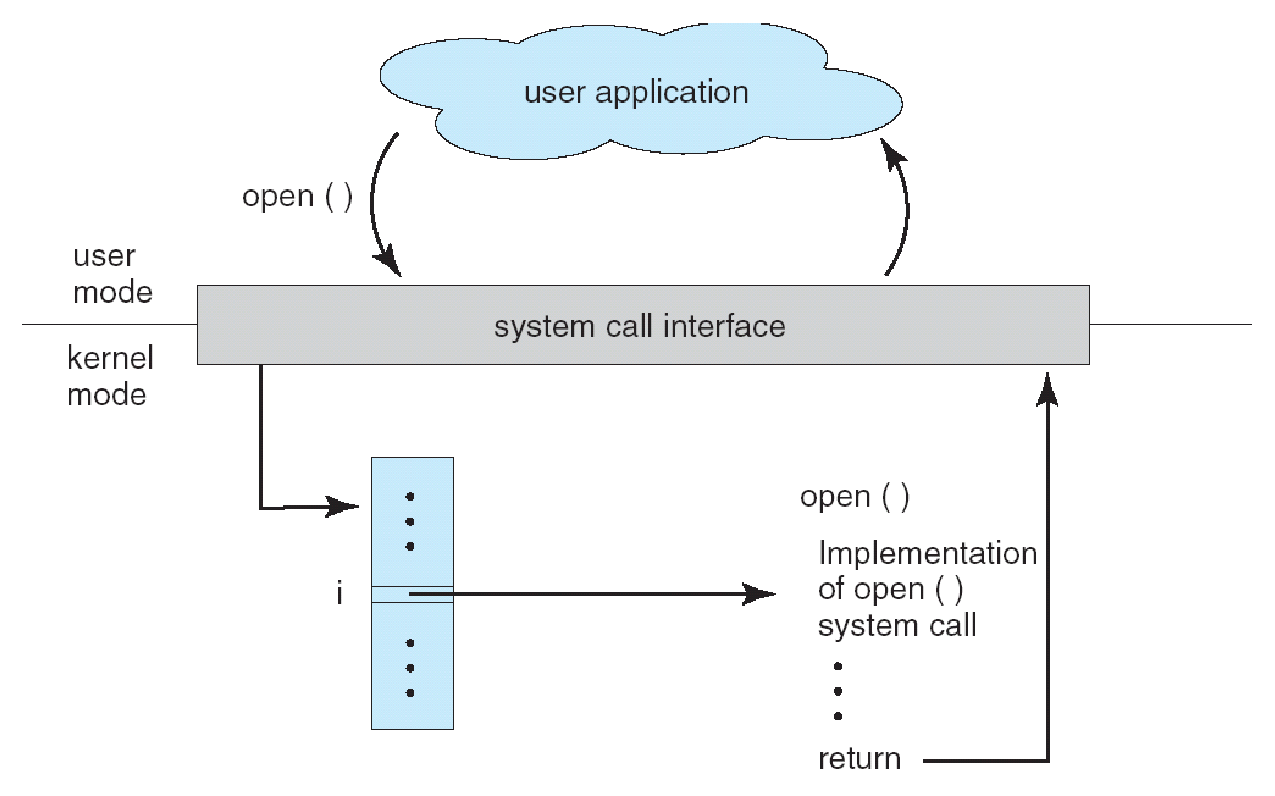
\includegraphics[height=2.3in]{figs/syscall}}
\itms{
  \item Applications can invoke kernel through \emph{system calls}
  \ittms{
  \item Special instruction transfers control to kernel
  \item \ldots which dispatches to one of few hundred syscall handlers
  }
}
\end{slide}

\begin{slide}{System calls (continued)}
\itms{
  \item Goal: Do things app.\ can't do in unprivileged mode
  \ittms{
    \item Like a library call, but into more privileged kernel code
  }
  %\item Applications request operations from kernel
  \item Kernel supplies well-defined \textit{system call} interface
  \ittms{
    \item Applications set up syscall arguments and \textit{trap} to kernel
    \item Kernel performs operation and returns result
  }
  \item Higher-level functions built on syscall interface
  \ittms{
    \item \texttt{printf, scanf, gets,} etc.\ all user-level code
  }
  \item Example: POSIX/UNIX interface
  \ittms{
    \item \texttt{open, close, read, write, \ldots}
  }
}
\end{slide}

\begin{slide}{System call example}
\centerline{\includegraphics[height=2.0in]{figs/libc}}
\itms{
  \item Standard library implemented in terms of syscalls
  \ittms{
    \item \emph{printf} -- in libc, has same privileges as application
    \item calls \emph{write} -- in kernel, which can send bits out
  serial port
  }
}
\end{slide}
\fi

\iffalse

\begin{slide}{UNIX file system calls}
\itms{
  \item Applications ``open'' files (or devices) by name
  \ittms{
    \item I/O happens through open files
  }
  \item \texttt{int open(char *path, int flags, /*mode*/...);}
  \ittms{
    \item \texttt{flags}: \texttt{O\_RDONLY}, \texttt{O\_WRONLY},
	\texttt{O\_RDWR}
    \item \texttt{O\_CREAT}: create the file if non-existent
    \item \texttt{O\_EXCL}: (w.\ \texttt{O\_CREAT}) create if file
exists already
    \item \texttt{O\_TRUNC}: Truncate the file
    \item \texttt{O\_APPEND}: Start writing from end of file
    \item \texttt{mode}: final argument with \texttt{O\_CREAT}
  }
  \item Returns file descriptor---used for all I/O to file
}
\end{slide}

\begin{slide}{Error returns}
\itms{
  \item What if \texttt{open} fails?  Returns -1 (invalid fd)
  \item Most system calls return -1 on failure
  \ittms{
    \item Specific kind of error in global int \texttt{errno}
  }
  \item \texttt{\#include <sys/errno.h>} for possible values
  \ittms{
    \item 2 = \texttt{ENOENT} ``No such file or directory''
    \item 13 = \texttt{EACCES} ``Permission Denied''
  }
  \item \texttt{perror} function prints human-readable message
  \ittms{
    \item \texttt{perror ("initfile");} \\
	$\to$ ``\texttt{initfile:\ No such file or directory}''
  }
}
\end{slide}

\begin{slide}{Operations on file descriptors}
\itms{
  \item \texttt{int read (int fd, void *buf, int nbytes);}
  \ittms{
    \item Returns number of bytes read
    \item Returns 0 bytes at end of file, or -1 on error
  }
  \item \texttt{int write (int fd, const void *buf, int nbytes);}
  \ittms{
    \item Returns number of bytes written, -1 on error
  }
  \item \texttt{off\_t lseek (int fd, off\_t pos, int whence);}
  \ittms{
    \item \texttt{whence}: 0 -- start, 1 -- current, 2 -- end
     \ittms{
       \item Returns previous file offset, or -1 on error
     }
  }
  \item \texttt{int close (int fd);}
%  \item \texttt{int fsync (int fd);}
%  \ittms{
%    \item Guarantee that file contents is stably on disk
%  }
}
\end{slide}

\begin{slide}{File descriptor numbers}
\itms{
  \item File descriptors are inherited by processes
  \ittms{
    \item When one process spawns another, same fds by default
  }
  \item Descriptors 0, 1, and~2 have special meaning
  \ittms{
  \item 0 -- ``standard input'' (\texttt{stdin} in ANSI C)
  \item 1 -- ``standard output'' (\texttt{stdout, printf} in ANSI C)
  \item 2 -- ``standard error'' (\texttt{stderr, perror} in ANSI C)
  \item Normally all three attached to terminal
  }
  \item Example:  \texttt{type.c}
  \ittms{
    \item Prints the contents of a file to \texttt{stdout}
  }
}
\end{slide}

\begin{slide}{\texttt{type.c}}
\begin{ccode}

     void
     typefile (char *filename)
     {
       int fd, nread;
       char buf[1024];

       fd = open (filename, O_RDONLY);
       if (fd == -1) {
         perror (filename);
         return;
       }

       while ((nread = read (fd, buf, sizeof (buf))) > 0)
         write (1, buf, nread);

       close (fd);
     }        
\end{ccode}
\end{slide}


\begin{slide}{Different system contexts}
\itms{
  \item A system is generally in one of several contexts
  \item \emph{User-level} -- CPU in user mode running application
  \item Kernel process context
  \ittms{
    \item Running kernel code on behalf of a particular process
    \item E.g., performing system call
    \item Also exception (mem.\ fault, numeric exception, etc.)
    \item Or executing a kernel-only process (e.g., network file server)
  }
  \item Kernel code not associated w.\ a process
  \ittms{
    \item Timer interrupt (hardclock)
    \item Device interrupt
    \item ``Softirqs'', ``Tasklets'' (Linux-specific terms)
  }
  \item Context switch code -- changing address spaces
  \item Idle -- nothing to do (might powerdown CPU)
}
\end{slide}

\begin{slide}{Transitions between contexts}
\itms{
  \item User $\to$ kernel process context:  {syscall, page fault}
  \item User/process context $\to$ interrupt handler:  {hardware}
  \item Process context $\to$ user/context switch:  {return}
  \item Process context $\to$ context switch:  {sleep}
  \item Context switch $\to$ user/process context
}
\end{slide}

\begin{slide}{CPU preemption}
\itms{
  \item Protection mechanism to prevent monopolizing CPU
  \item E.g., kernel programs timer to interrupt every 10 ms
  \ittms{
    \item Must be in supervisor mode to write appropriate I/O registers
    \item User code cannot re-program interval timer
  }
  \item Kernel sets interrupt to vector back to kernel
  \ittms{
    \item Regains control whenever interval timer fires
    \item Gives CPU to another process if someone else needs it
    \item Note: must be in supervisor mode to set interrupt entry points
    \item No way for user code to hijack interrupt handler
  }
  \item Result:  Cannot monopolize CPU with infinite loop
  \ittms{
    \item At worst get $1/N$ of CPU with $N$ CPU-hungry processes
  }
}
\end{slide}

\begin{slide}{Protection is not security}
\itms{
  \item How \emph{can} you monopolize CPU?
\pause
  \item Use multiple processes
  \item For many years, could wedge most OSes with
  \ittms{
    \item[] \texttt{int main() \char`\{\ while(1) fork(); \char`\}}
    \item Keeps creating more processes until system out of proc.\ slots
  }
  \item Other techniques: use all memory (\texttt{chill} program)
  \item Typically solved with technical/social combination
  \ittms{
    \item Technical solution:  Limit processes per user
    \item Social:  Reboot and yell at annoying users
    \item Social:  Pass laws (often debatable whether a good idea)
  }
}
\end{slide}

\begin{slide}{Address translation}
\itms{
  \item Protect memory of one program from actions of another
  \item Definitions
  \ittms{
    \item \emph{Address space}: all memory locations a program can name
    \item \emph{Virtual address}: addresses in process' address space
    \item \emph{Physical address}: address of real memory
    \item \emph{Translation}: map virtual to physical addresses
  }
  \item Translation done on every load and store
  \ittms{
    \item Modern CPUs do this in hardware for speed
  }
  \item Idea:  If you can't name it, you can't touch it
  \ittms{
    \item Ensure one process's translations don't include any other
          process's memory
  }
}
\end{slide}

\begin{slide}{More memory protection}
\itms{
  \item CPU allows kernel-only virtual addresses
  \ittms{
    \item Kernel typically part of all address spaces, \\
          e.g., to handle system call in same address space
    \item But must ensure apps can't touch kernel memory
  }
  \item CPU lets OS disable (invalidate) particular virtual addresses
  \ittms{
    \item Catch and halt buggy program that makes wild accesses
    \item Make virtual memory seem bigger than physical \\
          (e.g., bring a page in from disk only when accessed)
  }
  \item CPU enforced read-only virtual addresses useful
  \ittms{
    \item E.g., allows sharing of code pages between processes
    \item Plus many other optimizations
  }
  \item CPU enforced execute disable of VAs
  \ittms{
    \item Makes certain code injection attacks harder
  }
}
\end{slide}

\begin{slide}{Resource allocation \& performance}
\itms{
  \item Multitasking permits higher resource utilization
  \item Simple example:
  \ittms{
    \item Process downloading large file mostly waits for network
    \item You play a game while downloading the file
    \item Higher CPU utilization than if just downloading
  }
  \item Complexity arises with cost of switching
  \item Example:  Say disk 1,000 times slower than memory
  \ittms{
    \item 1 GB memory in machine
    \item 2 Processes want to run, each use 1 GB
    \item Can switch processes by swapping them out to disk
    \item Faster to run one at a time than keep context switching
  }
}
\end{slide}

\begin{slide}{Useful properties to exploit}
\itms{
  \item Skew
  \ittms{
    \item 80\% of time taken by 20\% of code
    \item 10\% of memory absorbs 90\% of references
    \item Basis behind cache: place 10\% in fast memory, 90\% in slow,
          usually looks like one big fast memory
  }
  \item Past predicts future (a.k.a.\ temporal locality)
  \ittms{
    \item What's the best cache entry to replace?
    \item If past $\approx$ future, then least-recently-used entry
  }
  \item Note conflict between fairness \& throughput
  \ittms{
    \item Higher throughput (fewer cache misses, etc.)\ to keep
          running same process
    \item But fairness says should periodically preempt CPU and give
          it to next process
  }
}
\end{slide}

\fi

\end{document}
